\documentclass[spanish,a4paper,11pt,twoside]{report}

%%%%%%%%%%%%%%%%%%%%%%%%%%%%%%%%%%%%%%%%%%%%%%%%%%%%%%%%%%%%%%%%%%%%%%%%%%%%%%%
\usepackage[dvips]{graphicx}
\usepackage[dvips]{epsfig}
\usepackage[latin1]{inputenc}
\usepackage[spanish]{babel}
\usepackage{alltt}
\usepackage{templates/algorithm}
\usepackage{templates/algorithmic}
\usepackage{templates/multirow}

%%%%%%%%%%%%%%%%%%%%%%%%%%%%%%%%%%%%%%%%%%%%%%%%%%%%%%%%%%%%%%%%%%%%%%%%%%%%%%%

\newcommand{\SONY}{{\sc Sony}}
\newcommand{\MICROSOFT}{{\sc Microsoft}}
\newcommand{\GCC}{\textsf{\textsc{G}CC}}
\newcommand{\INTEL}{\textsf{\textsc{I}ntel}}

%%% Traducimos el pseudocodigo
\renewcommand{\algorithmicwhile}{\textbf{mientras}}
\renewcommand{\algorithmicend}{\textbf{fin}}
\renewcommand{\algorithmicdo}{\textbf{hacer}}
\renewcommand{\algorithmicif}{\textbf{si}}
\renewcommand{\algorithmicthen}{\textbf{entonces}}
\renewcommand{\algorithmicrepeat}{\textbf{repetir}}
\renewcommand{\algorithmicuntil}{\textbf{hasta que}}
\renewcommand{\algorithmicelse}{\textbf{en otro caso}}
\renewcommand{\algorithmicfor}{\textbf{para}}

%\newcommand{\RETURN}{\textbf{retornar} }
\newcommand{\RET}{\STATE \textbf{retornar} }
\newcommand{\TO}{\textbf{hasta} }
\newcommand{\AND}{\textbf{y} }
\newcommand{\OR}{\textbf{o} }

%%%%%%%%%%%%%%%%% Creamos un entorno para listar c�digo fuente %%%%%%%%%%%%%%%
\newenvironment{sourcecode}
{\begin{list}{}{\setlength{\leftmargin}{1em}}\item\scriptsize\bfseries}
{\end{list}}

\newenvironment{littlesourcecode}
{\begin{list}{}{\setlength{\leftmargin}{1em}}\item\tiny\bfseries}
{\end{list}}

\newenvironment{summary}
{\par\noindent\begin{center}\textbf{Abstract}\end{center}\begin{itshape}\par\noindent}
{\end{itshape}}

\newenvironment{keywords}
{\begin{list}{}{\setlength{\leftmargin}{1em}}\item[\hskip\labelsep \bfseries Keywords:]}
{\end{list}}

\newenvironment{palabrasClave}
{\begin{list}{}{\setlength{\leftmargin}{1em}}\item[\hskip\labelsep \bfseries Palabras clave:]}
{\end{list}}


%%%%%%%%%%%%%%%%%%%%%%%%%%%%%%%%%%%%%%%%%%%%%%%%%%%%%%%%%%%%%%%%%%%%%%%%%%%%%%%
% Format
%%%%%%%%%%%%%%%%%%%%%%%%%%%%%%%%%%%%%%%%%%%%%%%%%%%%%%%%%%%%%%%%%%%%%%%%%%%%%%%

%%\topmargin -4 mm
%\topmargin -21 mm
%\headheight 10 mm
%\headsep 10 mm

%\textheight 229 mm
%\textheight 246 mm

%\oddsidemargin -5.4 mm
%\evensidemargin -5.4 mm
\oddsidemargin 5 mm
\evensidemargin 5 mm

%\oddsidemargin -3 mm
%\evensidemargin -3 mm

%\textwidth 17 cm
\textwidth 15 cm
%\columnsep 10 mm

\input{amssym.def}

%%%%%%%%%%%%%%%%%%%%%%%%%%%%%%%%%%%%%%%%%%%%%%%%%%%%%%%%%%%%%%%%%%%%%%%%%%%%%%%

\begin{document}

%%%%%%%%%%%%%%%%%%%%%%%%%%%%%%%%%%%%%%%%%%%%%%%%%%%%%%%%%%%%%%%%%%%%%%%%%%%%%%%
% First Page 
%%%%%%%%%%%%%%%%%%%%%%%%%%%%%%%%%%%%%%%%%%%%%%%%%%%%%%%%%%%%%%%%%%%%%%%%%%%%%%%

\pagestyle{empty}
\thispagestyle{empty}


\newcommand{\HRule}{\rule{\linewidth}{1mm}}
\setlength{\parindent}{0mm}
\setlength{\parskip}{0mm}
\vspace*{\stretch{1}}

\begin{center}

\includegraphics[width=0.2\textwidth]{images/logotipo-secundario-ULL}\\[0.25cm]
\end{center}

\HRule
\begin{center}
        {\Huge T�tulo del trabajo} \\[2.5mm] 
        {\Huge Subt�tulo} \\[2.5mm]
        {\Large Autor (o autores)} \\[5mm]
        {\Large \textit{Grupo ($1\mid2$) }} \\[5mm]


        {\em T�cnicas Experimentales. $1^{er}$ curso. $2^{do}$ semestre} \\[5mm]
        Lenguajes y Sistemas Inform�ticos \\[5mm]
        Facultad de Matem�ticas \\[5mm]
        
        Universidad de La Laguna \\
\end{center}
\HRule
\vspace*{\stretch{2}}
\begin{center}
  La Laguna, \today 
\end{center}

%%%%%%%%%%%%%%%%%%%%%%%%%%%%%%%%%%%%%%%%%%%%%%%%%%%%%%%%%%%%%%%%%%%%%%%%%%%%%%%

%%%%%%%%%%%%%%%%%%%%%%%%%%%%%%%%%%%%%%%%%%%%%%%%%%%%%%%%%%%%%%%%%%%%%%%%%%%%%%%
\newpage{\pagestyle{empty}\cleardoublepage}

\pagestyle{myheadings} %my head defined by markboth or markright
% No funciona bien \markboth sin "twoside" en \documentclass, pero al
% ponerlo se dan un mont�n de errores de underfull \vbox, con lo que no se
% ha puesto.
\markboth{Nombre del alumno}{T�tulo del trabajo}

%%%%%%%%%%%%%%%%%%%%%%%%%%%%%%%%%%%%%%%%%%%%%%%%%%%%%%%%%%%%%%%%%%%%%%%%%%%%%%%
%Numeracion en romanos
\renewcommand{\thepage}{\roman{page}}
\setcounter{page}{1}

%%%%%%%%%%%%%%%%%%%%%%%%%%%%%%%%%%%%%%%%%%%%%%%%%%%%%%%%%%%%%%%%%%%%%%%%%%%%%%%

\tableofcontents

%%%%%%%%%%%%%%%%%%%%%%%%%%%%%%%%%%%%%%%%%%%%%%%%%%%%%%%%%%%%%%%%%%%%%%%%%%%%%%%
\newpage{\pagestyle{empty}\cleardoublepage}

\listoffigures

%%%%%%%%%%%%%%%%%%%%%%%%%%%%%%%%%%%%%%%%%%%%%%%%%%%%%%%%%%%%%%%%%%%%%%%%%%%%%%%
\newpage{\pagestyle{empty}\cleardoublepage}

\listoftables

%%%%%%%%%%%%%%%%%%%%%%%%%%%%%%%%%%%%%%%%%%%%%%%%%%%%%%%%%%%%%%%%%%%%%%%%%%%%%%%
\newpage{\pagestyle{empty}\cleardoublepage}

%%%%%%%%%%%%%%%%%%%%%%%%%%%%%%%%%%%%%%%%%%%%%%%%%%%%%%%%%%%%%%%%%%%%%%%%%%%%%%%
%Numeracion a partir del capitulo I
\renewcommand{\thepage}{\arabic{page}}
\setcounter{page}{1}

\setlength{\parindent}{5mm}

%%%%%%%%%%%%%%%%%%%%%%%%%%%%%%%%%%%%%%%%%%%%%%%%%%%%%%%%%%%%%%%%%%%%%%%%%%%%%%%
\chapter{Motivaci�n y objetivos}
\label{chapter:obj}

%%%%%%%%%%%%%%%%%%%%%%%%%%%%%%%%%%%%%%%%%%%%%%%%%%%%%%%%%%%%%%%%%%%%%%%%%%%%%
% Chapter 1: Motivaci�n y Objetivos 
%%%%%%%%%%%%%%%%%%%%%%%%%%%%%%%%%%%%%%%%%%%%%%%%%%%%%%%%%%%%%%%%%%%%%%%%%%%%%%%

El objetivo de esta pr�ctica es demostrar los conocimientos adquiridos en Latex, Beamer y Python en el transcurso de la asignatura de T�cnicas Experimentales.
Aplicaremos los programas ya mencionados en la realizaci�n de un informe sobre la funci�n logaritmo neperiano y su desarrollo de Taylor.
Adem�s implementaremos un programa en Python que nos ayudar� a realizar varios experimentos para respaldar nuestras afirmaciones sobre el tema planteado.
%----------------------------------------------------------------------------------------------------
\section{Uso de Python,Beamer y Latex}
\label{1:sec:1}
\begin{itemize}
\item \LaTeX{} : Utilizaremos este programa en la realizaci�n del informe que presentaremos sobre $f(x)=Ln(x)$
\item Beamer : Recurriremos a la creaci�n de diapositivas para orientarnos en la exposici�n oral del trabajo.
\item Python : Crearemos un programa en lenguaje interpretado Python que utilizar� el desarrollo de Taylor para aproximar la funci�n Ln(x). 
As� como calcularemos el tiempo que tarda en realizar dicha aproximaci�n.
\end{itemize}
%---------------------------------------------------------------------------------






%%%%%%%%%%%%%%%%%%%%%%%%%%%%%%%%%%%%%%%%%%%%%%%%%%%%%%%%%%%%%%%%%%%%%%%%%%%%%%%
\chapter{Fundamentos te�ricos}
\label{chapter:teo}

%%%%%%%%%%%%%%%%%%%%%%%%%%%%%%%%%%%%%%%%%%%%%%%%%%%%%%%%%%%%%%%%%%%%%%%%%%%%%%%
% Chapter 2: Fundamentos Te�ricos 
%%%%%%%%%%%%%%%%%%%%%%%%%%%%%%%%%%%%%%%%%%%%%%%%%%%%%%%%%%%%%%%%%%%%%%%%%%%%%%%

%++++++++++++++++++++++++++++++++++++++++++++++++++++++++++++++++++++++++++++++

\section{Introducci�n}
\label{2:sec:1}
El desarrollo de Taylor calcula la aproximaci�n del valor de una funci�n centrada en un punto, as� como la estimaci�n del error. En este caso, investigaremos la funci�n logartimo Neperiano de ``x''.
Veremos la aproximaci�n y el error aplicando la serie de Taylor, y las variaciones de los resultados dependiendo de las constantes que fijemos. Adem�s, nos introduciremos en el tema hablando de la historia
del desarrollo de Taylor y del Logaritmo Neperiano.
Para ello utilizaremos tal y como hemos mencionado anteriormente,el lenguaje de programaci�n Python elaborando programas que respalden las hip�tesis dadas y nos aporte el resultdo esperado. 
%------------------------------------------------------------------------------------
\section{Historia}
\label{2:sec:2}
El fil�sofo griego Zen�n fue uno de los primero en considera el problema de la suma de una serie infinita para obtener un resultado finito, tras varios estudios la consider� imposible,
como resultado surgi� la paradoja de Zen�n. M�s tarde, Arist�teles propuso una resoluci�n filos�fica a la paradoja.Su contenido matem�tico no fue resuelto hasta que lo retomaron Dem�crito y Arqu�medes 
a trav�s del m�todo de agotamiento de Arqu�medes, que se basa en que un n�mero infinito podr�a expresarse finalmente mediante un resultado finito.

En el siglo XIV, Madhava de Sangamagrama dio los primeros ejemplos de la utilizaci�n de la serie de Taylor y otros m�todos relacionados; aunque no queda constancia de sus estudios, los 
escritos posteriores de matem�ticos de la India sugieren que encontr� algunos casos especiales de la serie de Taylor,como por ejemplo las funciones trigonom�tricas. 
Las series de Taylor tuvo gran relevancia en los estudios que realizaba la famosa escuela de Kerala de astronom�a y matem�ticas.
\clearpage
En el siglo XVII, James Gregory trabaj� en esta �rea y public� varias series de Taylor centradas en el punto cero. Sin embargo, no fue hasta el siglo XVIII cuando se present� de manera formal el Desarrollo de Taylor que proporcionaba 
una soluci�n finita para cualquier tipo de funci�n. Esta aportaci�n fue dada en 1715 por el matem�tico brit�nico Brook Taylor (1685-1731).
 \[\theta = \tan \theta - (1/3) \tan^3 \theta + (1/5) \tan^5 \theta - \cdots,\,\]
 
 
\footnote{Gregory redescubri� un teorema originalmente formulado por el matem�tico indio Madhava de Sangamagrama, la serie del arcotangente}

\begin{figure}[!th]
\begin{center}

\includegraphics[width=0.25\textwidth]{images/taylor.eps}
\caption{Brook Taylor}
\label{fig:1}
\end{center}
\end{figure}
 
El teorema de Taylor da estimaciones cuantitativas sobre el error en la aproximaci�n de una funci�n. Cualquier n�mero finito de t�rminos iniciales de la serie de Taylor de una funci�n se llama
polinomio de Taylor. La serie de Taylor de una funci�n es el l�mite de los polinomios de Taylor de esa funci�n, siempre que el l�mite existe. Una funci�n no puede ser igual a su serie 
de Taylor, aunque su serie de Taylor converge en cada punto. Una funci�n que es igual a su serie de Taylor en un intervalo abierto se conoce como una funci�n anal�tica.
Es importante mencionar que si aplicamos la Serie de Taylor en el punto ``0'', la serie se llamar�a Desarrollo de Maclaurin expresada de la siguiente manera:
 \[f(x)=f(0)+f^1(0)x+\frac{f^2(0)}{2!}x^2+\frac{f^3(0)}{3!}x^3+...+\frac{f^n(0)}{n!}x^n\]
Donde:
\begin{center}
\begin{itemize}
\item ``x'' es el punto.
\item ``0'' es el centro.
\item ``n'' es el grado.
\end{itemize}
\end{center}
%---------------------------------------------------------------------------------------
\section{Serie de Taylor y Logaritmo Neperiano}
\label{2:sec:3}
\subsection{Series de potencias: Taylor}
En matem�ticas, una serie de Taylor es una representaci�n de una funci�n como una infinita suma de t�rminos que se calculan a partir de las derivadas de la funci�n para un determinado valor de la variable.
Para analizar el comportamiento de una funcion ``f'' en las proximadades de un punto `a',podemos recurrir a la aproximaci�n local cerca de dicho punto. De esta manera,podr�amos sacar conclusiones sobre el
comportamiento de la funci�n en el punto `a'.
Los resultados que se obtengan ser�n tanto m�s precisos cuanto mayor sea la aproximaci�n que se maneje cerca del punto en cuesti�n.
\subsection{Logaritmo Neperiano}
Estudiando los fen�menos de creciemiento y decrecimiento en la naturaleza, se observ� que con frecuencia aprec�an potencias de un n�mero irracional al que se llamo ``e'', 
cuyo valor aproximado es:
 \[ e \approx 2,7182818284590452353602874713527. \] 

Para estudiar estos fen�menos se aplicaban los logaritmos y sus propiedades, en concreto el logaritmo en base ``e'', tambi�n llamado ``logaritmo neperiano''. 
\[ln(x)=log_e(x)\]
 
\section{Aplicaci�n matem�tica del Teorema de Taylor y uso del Logaritmo neperiano}
\label{2:sec:4}
Sea f una funci�n sufcientemente regular y x la variable, podemos aproximar la funci�n, para x cerca de a, mediante polinomios denominados polinomios de Taylor cuya expresi�n es la siguiente:


  \[ P_{(n,a)} = f(a)+\frac{f'(a)}{1!}(x-a)+\frac{f''(a)}{2!}(x-a)^2+\frac{f^{(3)}(a)}{3!}(x-a)^3+\cdots \frac{f^{(n)}(a)}{n!} (x-a)^{n}\,. \]
  
Donde la derivada de orden cero de la funci�n es definida como la propia funci�n, ``$n!$'' es el factorial de ``n'' y  $f^{(n)}.(a)$ denota la n-�sima derivada de f para el valor a.
Adem�s,es importante mencionar que si a=0, la serie se denomina Serie de Maclaurin. 
\clearpage
\emph{}
\subsection{Aplicaci�n Series de Taylor en f(x)=ln(x)}
Se aplica el desarrollo de Taylor de manera general, donde:
\[n=grado\]
\[a=valor\]
\[f^t(a)= \frac{b}{a^t},\]
\small{\[1<t<n\]}

Sea f(x)=ln(x) :

\begin{enumerate}
\item Se calcula la imagen:
f(a) = ln(a)
\item Se calcula la primera derivada y su imagen:
$f'(a) = \frac{1}{a}$ 
\item Se calcula la segunda derivada y su imagen:
$f''(a) = \frac{-1}{a^2}$
\item Se calcula la tercera derivada y su imagen:
$f'''(a) = \frac{2}{a^3}$
\item Calculamos la en�sima derivada y su imagen:
$f^n(a) = \frac{(n-1).(-b)}{a^{(n)}}\,.$
\end{enumerate}

Entonces,

\[ P_{(n,a)} = ln(a)+\frac{\frac{1}{a}}{1!}(x-a)+\frac{\frac{-1}{a^2}}{2!}(x-a)^2+\frac{\frac{2}{a^3}}{3!}(x-a)^3+\cdots \frac{ \frac{(n-1).(-b)}{a^{(n)}}}{n!} (x-a)^{n}\,. \]

 

%%%%%%%%%%%%%%%%%%%%%%%%%%%%%%%%%%%%%%%%%%%%%%%%%%%%%%%%%%%%%%%%%%%%%%%%%%%%%%%
\chapter{Procedimiento experimental}
\label{chapter:exp}

%%%%%%%%%%%%%%%%%%%%%%%%%%%%%%%%%%%%%%%%%%%%%%%%%%%%%%%%%%%%%%%%%%%%%%%%%%%%%%%
% Chapter 3: Procedimiento experimental 
%%%%%%%%%%%%%%%%%%%%%%%%%%%%%%%%%%%%%%%%%%%%%%%%%%%%%%%%%%%%%%%%%%%%%%%%%%%%%%%



%++++++++++++++++++++++++++++++++++++++++++++++++++++++++++++++++++++++++++++++
\section{Descripci�n de los experimentos}
\label{3:sec:1}
Tras elaborar un programa en Python capaz de calcular la aproximaci�n de la funci�n ln(x) mediante la serie de Taylor y el tiempo que tarda la m�quina en realizar esa aproximaci�n,
hemos realizado varios experimentos fijando el punto,el centro o el grado. Adem�s,tambi�n elaboramos un programa que nos calcula el error de dicha aproximaci�n.
Los experimentos realizados son los siguientes: 
\begin{enumerate}
\item Fijamos el grado de la Serie de Taylor(n=10),el punto en el que deseamos que se aplique (x=4) y variamos el centro.
\item Fijamos el grado de la Serie de Taylor (n=8), el centro (c=6) y variamos el punto en el que deseamos que se aplique.
\item Fijamos el centro(c=1) , el punto en el que deseamos que se aplique la aproximaci�n (x=2) y variamos el grado.
\end{enumerate}
%++++++++++++++++++++++++++++++++++++++++++++++++++++++++++++++++++++++++++++++
\section{Descripci�n del material}
\label{3:sec:2}
Todos los experimentos realizados se han llevado a cabo en un ordenador con las siguientes caracter�sticas:
\begin{verbatim}
 - Sistema operativo : Linux, Ubuntu.
 - Procesador: Intel(R) Core(TM) i3 
 - CPU :  M 350  @ 2.27GHz 
\end{verbatim}
\clearpage
%++++++++++++++++++++++++++++++++++++++++++++++++++++++++++++++++++++++++++++++
\section{Resultados obtenidos}
\subsection{Funci�n real del Logartimo Neperiano}
\begin{figure}[!th]

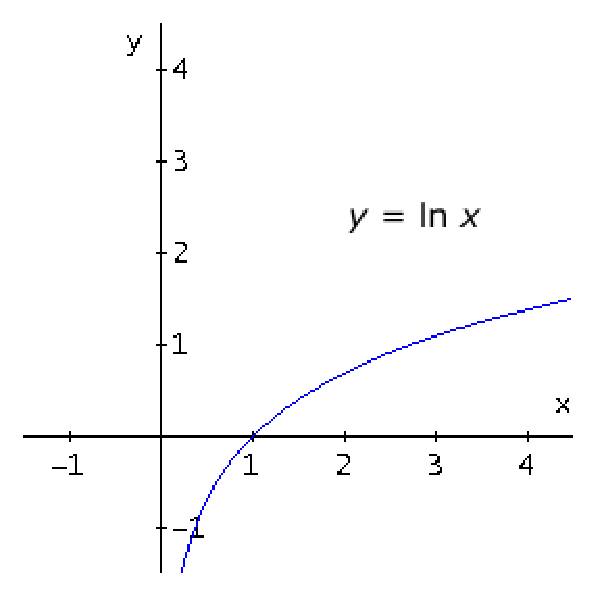
\includegraphics[width=0.30\textwidth]{images/fun053.eps}
\caption{Funci�n Logaritmo Neperiano}
\label{fig:1}

\end{figure}
\label{3:sec:3}

\subsection{Variaci�n del centro}
Fijando n=10 y x=4

\begin{tabular}{|l | r@{,}l |}
\hline
Si el valor de c= 2   & 1  & 33878210119487\\
\hline
Si el valor de c= 3   & 1  & 38629396788690\\
\hline 
Si el valor de c= 5   & 1  & 38629436340045\\
\hline
Si el valor de c= 30  & 1  & 48572417754861\\
\hline
Si el valor de c= 60  & 1  & 74292118557045\\
\hline
\end{tabular}


\subsection{Variaci�n del punto }
Fijando n=8 y c=6

\begin{tabular}{|l | r@{,}l |}
\hline
Si el valor de x= 8  &  2 & 07943719692636\\
\hline
Si el valor de x= 7  &  1 & 94591013946629\\
\hline
Si el valor de x= 6  &  1 & 79175946922805\\
\hline
Si el valor de x = 5 &  1 & 60943792540920\\
\hline
Si el valor de x= 4  & 1  & 38630243959407\\
\hline
\end{tabular}

\subsection{Variaci�n del grado }
Fijando x=2 y c=1

\begin{tabular}{|l | r@{,}l |}
\hline
Si el valor de n= 5     &  0 & 783333333333333\\
\hline
Si el valor de n= 15    &  0 & 725371850371850\\
\hline
Si el valor de n= 25    &  0 & 712747499542829\\
\hline
Si el valor de n= 200   &  0 & 690653430481824\\
\hline
Si el valor de n= 800   &  0 & 692522571184642\\
\hline
\end{tabular}

\clearpage
\subsection{Tiempo }
Tomamos los resultados de la tabla anterior y calculamos el tiempo que tarda el ordenador en obtener los resultados.

\begin{tabular}{|l | r@{,}l |}
\hline
Si el valor de n= 5     &  9 & 53674316406e-07\\
\hline
Si el valor de n= 15    &  9 & 53674316406e-07\\
\hline
Si el valor de n= 25    &  9 & 53674316406e-07\\
\hline
Si el valor de n= 200   &  1 & 19209289551e-06\\
\hline
Si el valor de n= 800   &  1 & 90734863281e-06\\
\hline

\end{tabular}
%------------------------------------------------------------------------------

%------------------------------------------------------------------------------

%++++++++++++++++++++++++++++++++++++++++++++++++++++++++++++++++++++++++++++++
\section{An�lisis de los resultados}
\label{3:sec:4}

\begin{itemize}
\item Variaci�n del centro: Variando el centro, fijando el grado (n=10) y el punto (x=4), podemos observar que cuanto m�s se aleja centro del punto menos acertado es el resultado.
\item Variaci�n del punto: Variando el punto, y fijando el centro (c=6) y el grado (n=8), observamos que si el punto es igual al centro el valor de la Serie de Taylor es  no conduce a ning�n error, ya que al ser iguales su diferencia es cero 
y nos da la imagen en ese punto o centro del logaritmo neperiano. Adem�s, vemos que si incrementamos la diferencia entre ambos puntos el resultado se aleja m�s del aut�ntico valor.
\item Variaci�n del grado: Al variar el grado y fijando el punto (x=2) y el centro (c=2), apreciamos que cuanto mayor es el grado m�s disminuye el error, por lo cual, si aunmentamos el valor del grado m�s precisos son los resultados. 
\item Tiempo: en cuanto al tiempo, el ordenador realiza los procesos m�s lento dependiendo del grado, ya que la ecuaci�n es m�s larga.
\end{itemize}


%%%%%%%%%%%%%%%%%%%%%%%%%%%%%%%%%%%%%%%%%%%%%%%%%%%%%%%%%%%%%%%%%%%%%%%%%%%%%%%
\chapter{Conclusiones}
\label{chapter:conclusiones}

%%%%%%%%%%%%%%%%%%%%%%%%%%%%%%%%%%%%%%%%%%%%%%%%%%%%%%%%%%%%%%%%%%%%%%%%%%%%%
% Chapter 4: Conclusiones y Trabajos Futuros 
%%%%%%%%%%%%%%%%%%%%%%%%%%%%%%%%%%%%%%%%%%%%%%%%%%%%%%%%%%%%%%%%%%%%%%%%%%%%%%%

bla, bla, bla, etc.


%%%%%%%%%%%%%%%%%%%%%%%%%%%%%%%%%%%%%%%%%%%%%%%%%%%%%%%%%%%%%%%%%%%%%%%%%%%%%%%

%%%%%%%%%%%%%%%%%%%%%%%%%%%%%%%%%%%%%%%%%%%%%%%%%%%%%%%%%%%%%%%%%%%%%%%%%%%%%%%
\newpage{\pagestyle{empty}\cleardoublepage}
\thispagestyle{empty}
\begin{appendix}

\chapter{T�tulo del Ap�ndice 1}
\label{appendix:1}

\section{Algoritmo XXX}
\label{Apendice1:XXX}

\begin{center}
\begin{footnotesize}
\begin{verbatim}
###################################################################################
# Fichero .py
###################################################################################
#
# AUTORES
#   
# FECHA
#
# DESCRIPCION
#
###################################################################################
\end{verbatim}
\end{footnotesize}
\end{center}

\section{Algoritmo YYY}
\label{Apendice1:YYY}

\begin{center}
\begin{footnotesize}
\begin{verbatim}
/###################################################################################
 # Fichero .h
 ###################################################################################
 #
 # AUTORES
 #
 # FECHA
 #
 # DESCRIPCION
 #
 ##################################################################################
\end{verbatim}
\end{footnotesize}
\end{center}


\chapter{T�tulo del Ap�ndice 2}
\label{appendix:2}

\section{Otro apendice: Seccion 1}
\label{Apendice2:label}

\begin{center}
\begin{footnotesize}

\begin{verbatim}
Texto
\end{verbatim}

\end{footnotesize}
\end{center}

\section{Otro apendice: Seccion 2}
\label{Apendice2:label2}

\begin{center}
\begin{footnotesize}

\begin{verbatim}
Texto
\end{verbatim}


\end{footnotesize}
\end{center}


\end{appendix}

%%%%%%%%%%%%%%%%%%%%%%%%%%%%%%%%%%%%%%%%%%%%%%%%%%%%%%%%%%%%%%%%%%%%%%%%%%%%%%%
\addcontentsline{toc}{chapter}{Bibliograf�a}
\bibliographystyle{plain}


\bibliography{bib/references}
\nocite{*}

%%%%%%%%%%%%%%%%%%%%%%%%%%%%%%%%%%%%%%%%%%%%%%%%%%%%%%%%%%%%%%%%%%%%%%%%%%%%%%%

\end{document}
